\section{Preliminary}\label{sec:preliminary}

\rev{Before discussing the system design for neural network acceleration, we first introduce the basic concepts of neural networks and the basic components of an FPGA-based accelerator design.}

\subsection{Neural Network}

\begin{figure}[ht]
    \centering
    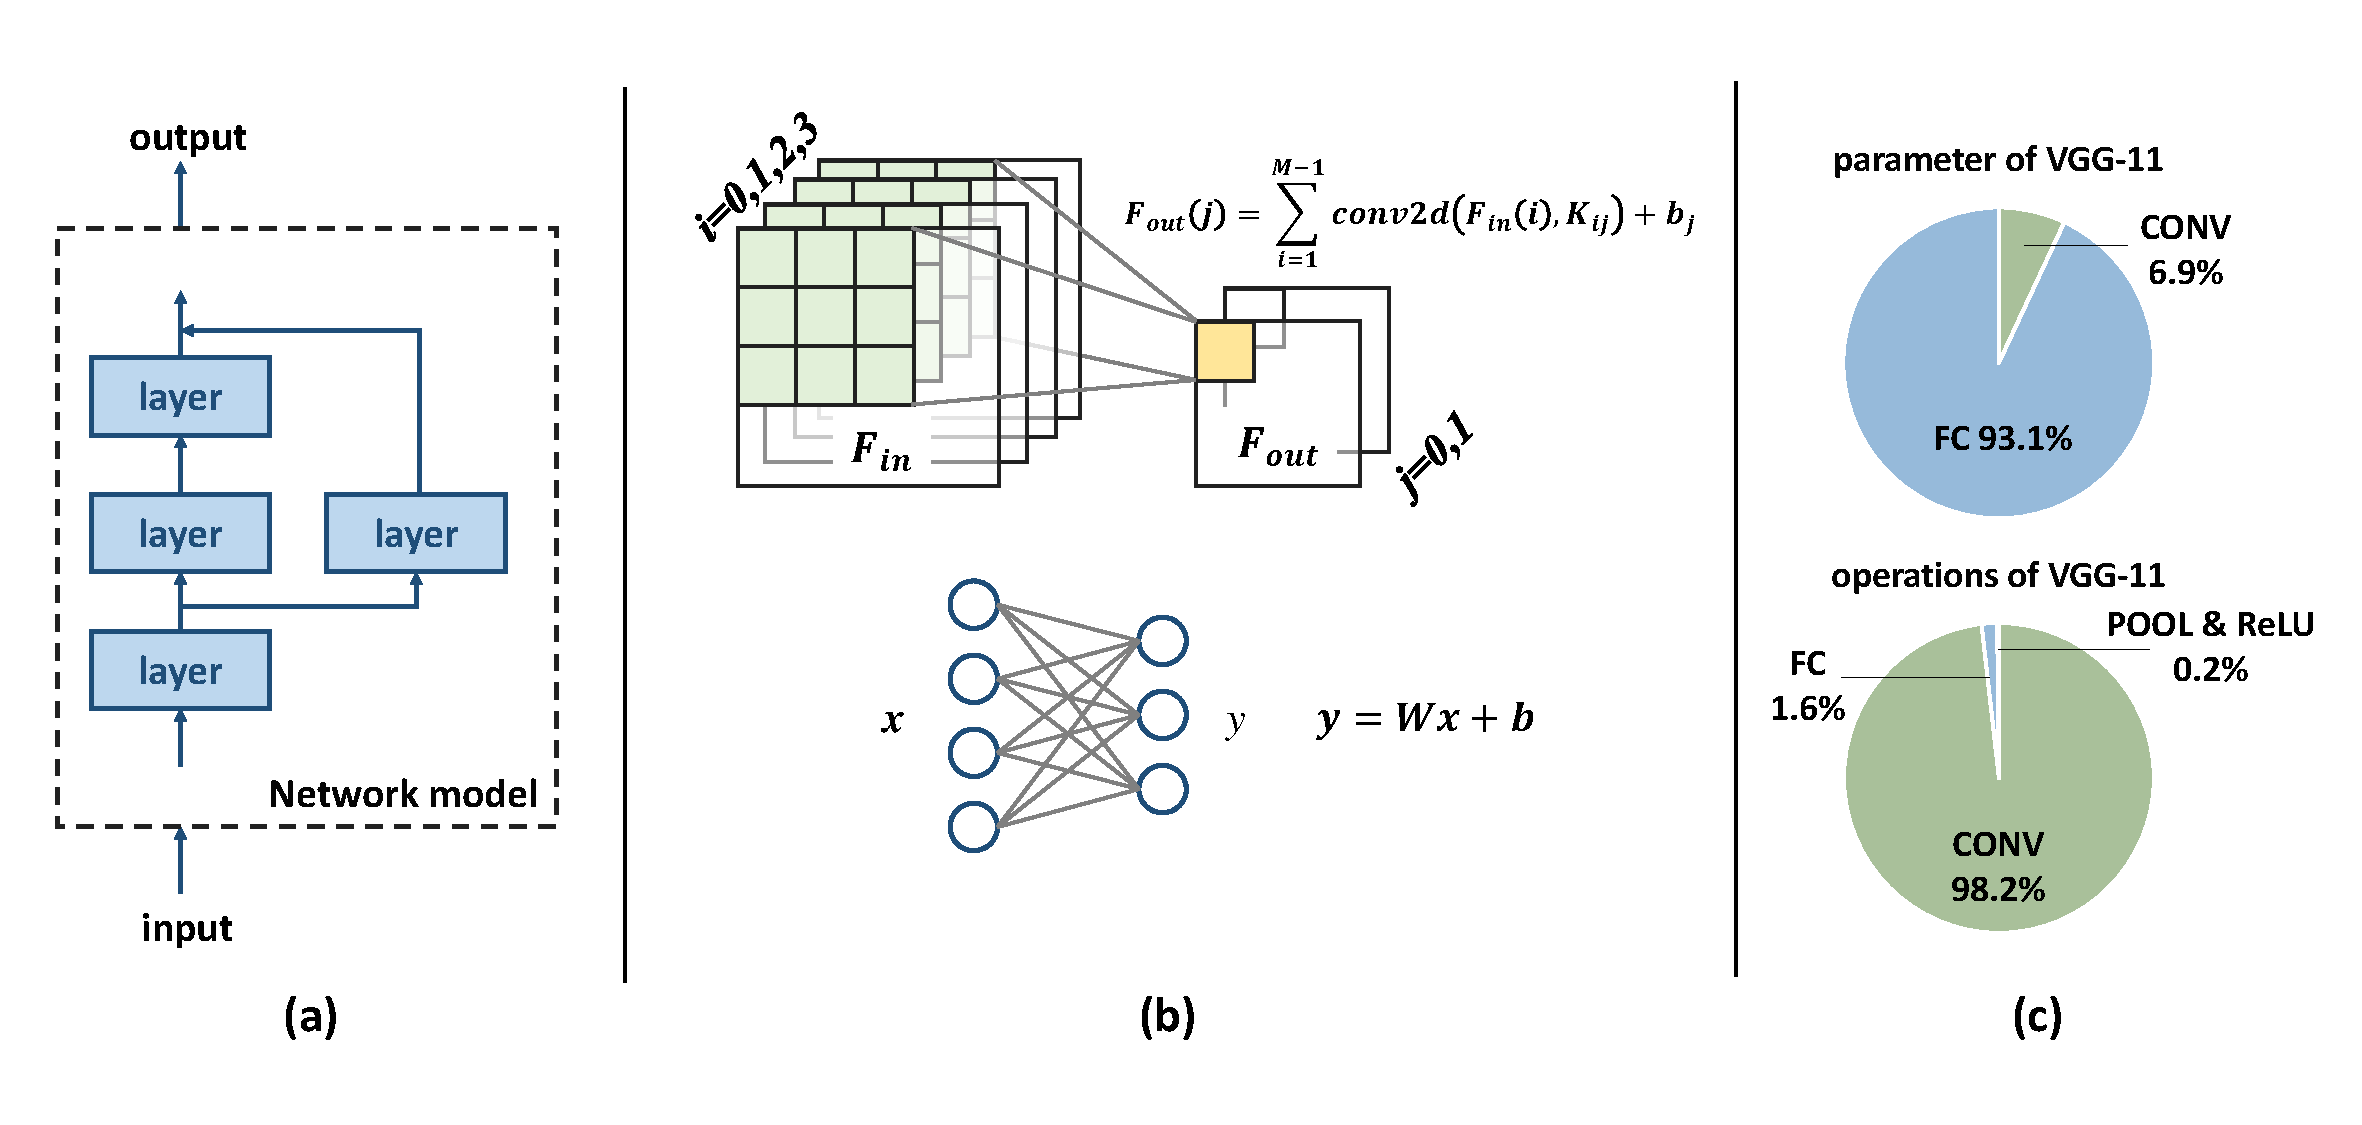
\includegraphics[width=1.0\columnwidth]{fig/cnn_preliminary.pdf}
    \caption{\rev{(a) Computation graph of a neural network model. (b) CONV and FC layers in NN model. (c) CONV and FC layers dominates the computation and parameter of a NN model.}}
    \label{fig:cnn_preliminary}
\end{figure}

\rev{In this section, we introduce the basic functions in a neural network. A neural network model can be described as a directed graph shown in Figure~\ref{fig:cnn_preliminary}(a). Each vertex of the graph denotes a layer which conducts operations on data from a previous layer or input and generates results to the next layer or output.

Convolution (CONV) layers and fully connected (FC) layers are two common types of layers in NN models. The functions of these two layers are shown in Figure~\ref{fig:cnn_preliminary}(b). CONV layers conduct 2D convolutions on a set of input feature maps $F_{in}$ and add the results to get output feature maps $F_{out}$. FC layers receives a feature vector as input and conduct matrix-vector multiplications.

Besides CONV and FC layers, NN layers also have pooling, ReLU~\cite{krizhevsky2012imagenet}, concat~\cite{szegedy2015going}, element-wise~\cite{he2016deep} and other types of layers. But these layers contributes little to the computation and storage requirement of a neural network model. Figure~\ref{fig:cnn_preliminary}(c) shows the distribution of parameter and operations in the VGG-11 model~\cite{simonyan2014very}. CONV and FC layers together contributes more than 99\% of the network's parameters and operations. So most of the neural network acceleration systems focus on these two types of layers.
}

\subsection{FPGA-based Accelerator}

\rev{Recent years, FPGA is becoming a promising solution for accelerating certain algorithms. Compared with CPU, GPU, and DSP platforms, for which the software and hardware are designed independently, FPGA enables the developers to implement only the necessary logic in hardware according to the target algorithm. By eliminating the redundancy in hardware, FPGA is able to achieve higher efficiency. Similar to FPGA, application specific integrated circuit (ASIC) 

For FPGA-based neural network accelerator, a typical architecture of the system is shown in Figure~\ref{}.}